% !TEX encoding = UTF-8 Unicode
%!TEX TS-program = xelatex

\documentclass[12pt]{extarticle}
% extarticle is like article but can handle 8pt, 9pt, 10pt, 11pt, 12pt, 14pt, 17pt, and 20pt text

\def \ititle {Origins of Mind}
 
\def \isubtitle {Lecture 08}
 
\def \iauthor {Stephen A. Butterfill}
\def \iemail{s.butterfill@warwick.ac.uk}
\date{}

%for strikethrough
\usepackage[normalem]{ulem}

\usepackage{pdfpages}


\input{$HOME/Documents/submissions/preamble_steve_handout}

%logic symbol \leftmodels
\usepackage{MnSymbol}

%\bibpunct{}{}{,}{s}{}{,}  %use superscript TICS style bib
%remove hanging indent for TICS style bib
%TODO doesnt work
\setlength{\bibhang}{0em}
%\setlength{\bibsep}{0.5em}


%itemize bullet should be dash
\renewcommand{\labelitemi}{$-$}

\begin{document}

%\raggedcolumns

\begin{multicols*}{3}

\setlength\footnotesep{1em}


\bibliographystyle{newapa} %apalike

%\maketitle
%\tableofcontents




%--------------- 
%--- start paste
\def \ititle {Logic (PH133)}
 
\def \isubtitle {Lecture 5}
 
\begin{center}
 
{\Large
 
\textbf{\ititle}: \isubtitle
 
}
 
 
 
\iemail %
 
\end{center}
 
 
 
 
\section{Not Or}
 
\emph{Reading:} §3.7
 
\begin{center}
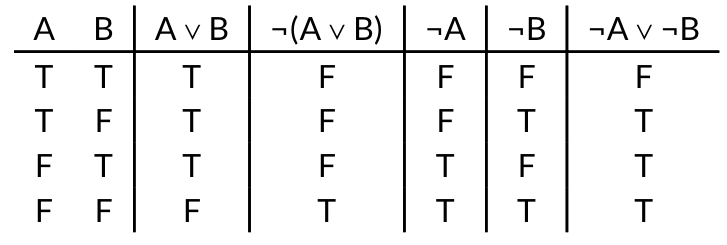
\includegraphics[scale=0.3]{img/tt_unit_603.png}
\end{center}
 
 
\section{What does ‘→’ mean?}
 
\emph{Reading:} §7.1
 
Assuming that the rules of Fitch are such that it is impossible to prove an argument which is not logically valid, the truth table for → is fixed if we accept →Elim and →Intro.
 
How do the rules of proof for → fix its truth table?
 
\begin{center}
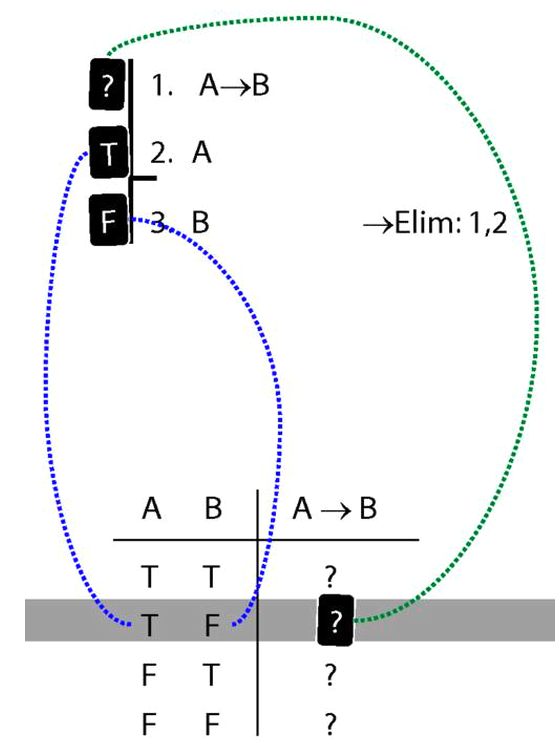
\includegraphics[scale=0.3]{img/unit_700_rule_to_tt.png}
\end{center}
 
 
\section{I Met a Philosopher}
 
\emph{Reading:} §9.2, §9.3, §9.5
 
 
 
 
 
 
\section{What does ∀ mean?}
 
\emph{Reading:} §9.4
 
We give the meaning of ∀ by specifying what it takes for a sentence containing ∀ to be true:
 
\begin{enumerate}
 
\item Give every object a name.
 
\item For each name in turn, create a new sentence like this: delete the quantifier and replace all instances of the variable it binds with that name.
 
\item If ALL of the new sentences are true, so is the original sentence.
 
\end{enumerate}
 
 
 
\section{Vegetarians Are Evil}
 
\emph{Reading:} §9.2, §9.3, §9.5
 
\begin{center}
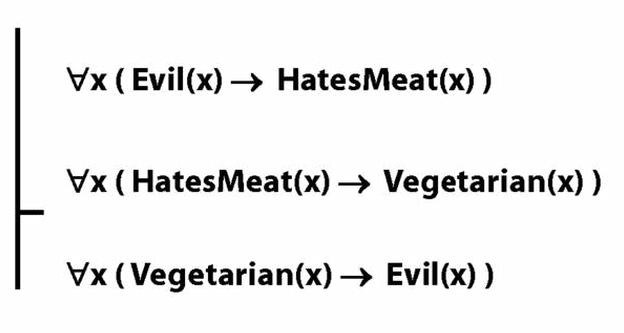
\includegraphics[scale=0.3]{img/vegetarians.png}
\end{center}
 
 
\section{Counterexamples with Quantifiers}
 
\begin{center}
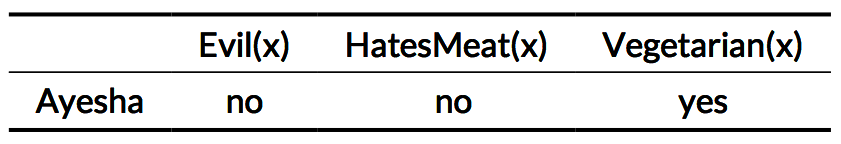
\includegraphics[scale=0.3]{img/unit_502b_counterexample.png}
\end{center}
 
 
\section{Not If}
 
\begin{center}
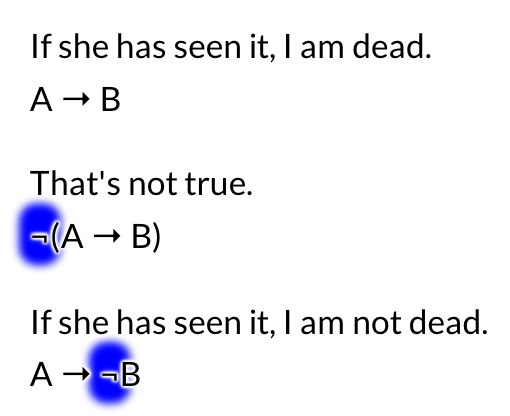
\includegraphics[scale=0.3]{img/not_if.png}
\end{center}
\begin{center}
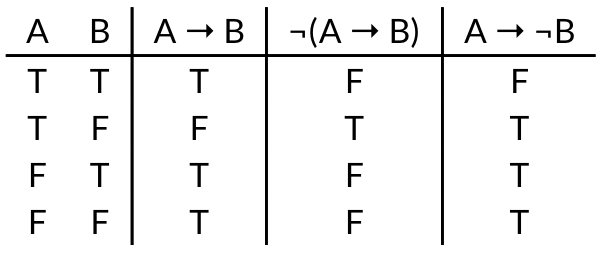
\includegraphics[scale=0.3]{img/not_if_tt.png}
\end{center}
 
 
\section{↔ : truth tables and rules}
 
\begin{center}
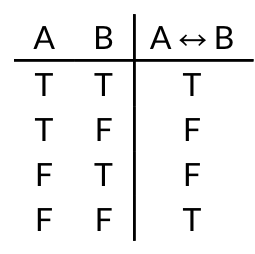
\includegraphics[scale=0.3]{img/tt_biconditional.png}
\end{center}
\begin{center}
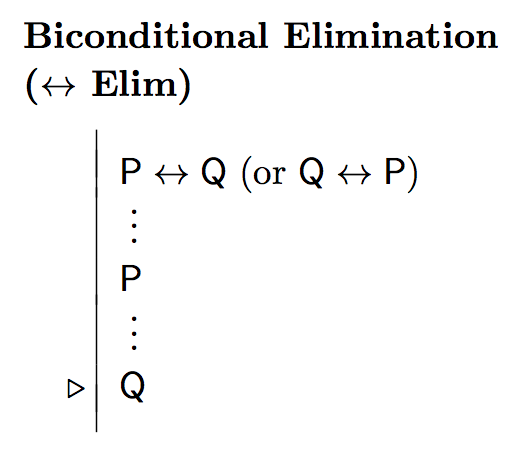
\includegraphics[scale=0.3]{img/rule_biconditional_elim.png}
\end{center}
\begin{center}
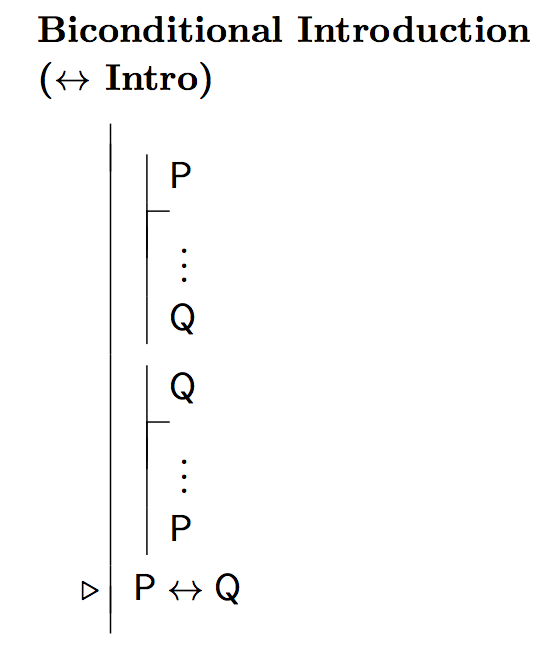
\includegraphics[scale=0.3]{img/rule_biconditional_intro.png}
\end{center}
 
\columnbreak
\section{Does ‘if’ mean what ‘→’ means?}
 
\emph{Reading:} §7.3
 
\begin{minipage}{\columnwidth}
 
These two arguments are valid: does that mean that `if' means what `→' means?
 
\begin{center}
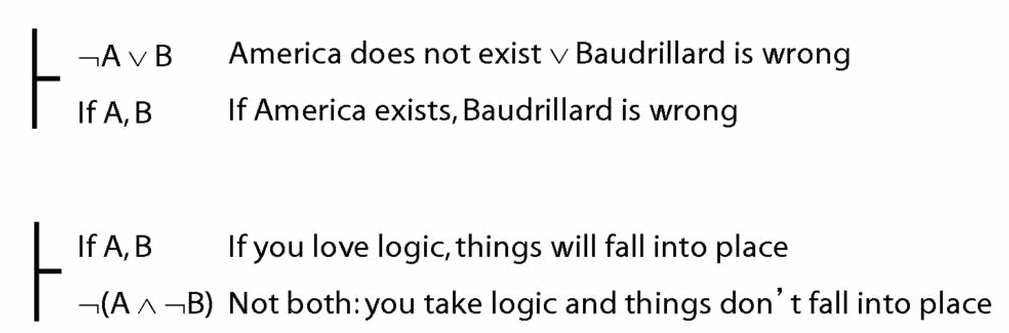
\includegraphics[scale=0.3]{img/if_is_arrow.png}
\end{center}
\end{minipage}
 
\begin{minipage}{\columnwidth}
 
The English argument isn't valid; the FOL argument is valid; therefore `if' can't mean what `→' means?
 
\begin{center}
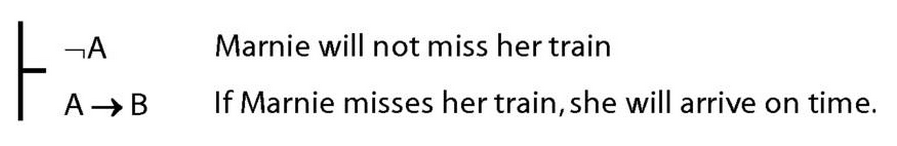
\includegraphics[scale=0.3]{img/if_aint_arrow.png}
\end{center}
\end{minipage}
 %--- end paste
%--------------- 
 


\end{multicols*}

\end{document}